% Chapter Template

\chapter{Dataset and Exploratory Analysis} % Main chapter title

\label{c3} % Change X to a consecutive number; for referencing this chapter elsewhere, use \ref{ChapterX}

%----------------------------------------------------------------------------------------
%	SECTION 1
%----------------------------------------------------------------------------------------
\section{Data Acquisition and Pre-processing}
Data has been acquired through Kaggle. It is one of the famous Rossmann Store Sale \cite{sazontyevrossmann} data where several papers already been published through different publishing entities. Rossmann Dataset have consecutive three years of sales data between 2013-01 and 2015-07. It has more than 8 lakhs of samples after eliminating null and zero values from sales feature. The data consists of 1115 stores. The available data is multivariate in nature, but sales contribution is not much dependent on all features \cite{kim2019bilstm}. It needs to be analysed and predicted on the available parameters by ML Model to get valuable insights of data as well as an optimized results by the models based on different performance parameters like RMSE and MAPE. The correlation of stores have been taken into consideration for minimizing. The prediction of data is seriously affected by data quality therefore, it plays a decisive role in analysis. Since, there is a lot of stores present, so for the sake of convenience, we have taken those stores whose sales correlation is less than 2.0 with other stores and hence we have taken sorted ten stores sales data based on Mean Correlation Value ( MCV ) of store correlations. Correlation \cite{habets2009new} has been taken for the relative behaviour of different stores sales data. Highly correlated feature generally behaves identically and hence it is not necessary to analyse them as a different entity, instead any single feature will be enough to define as a whole. 

Under pre-processing, null values, usually due to weekend or holidays from store data, are eliminated. The feature \textit{Stateholiday} consisting of several holiday due to some occasions mentioned as in the form of $\{a,b,c\}$ in the data observations, are further transformed to $\{0,1,2\}$ respectively. In terms of carrying operation for outliers \cite{kwak2017statistical}, the data has been kept as it is because sometimes, it might reduce the information on elimination or appears useful for the models used for the data \cite{toochaei2023evaluating}. The outliers may be visually observed using some of the plot visualizations like boxplot, violin plot etc. The enhancement of features from the data is performed through feature engineering, to inspect and analyse the responses of different views from the dataset with extended features $X’$. Further, data is splited into train and test data within a fixed range of time slot. In our case, values after “2014-12”, is taken as test data which is within the range of 20\% to 30\% of whole data. After data split, the Multiview Construction of data is taken into account by the introducing Random Feature Set Partitioning (RFSP) \cite{kumar2023review} approach for the data. Although, RFSP method has its own significance as well as limitations in relevance with multi-view construction. Taking the limitation part, it eventually may take same value multiple times and neglecting the most relevant features as well, that may lead to poor performance in learning the model. The performance of proposed framework is comparatively analysed based on used performance metric.
This approach is quite supportive towards operating data having large number of features. The set of stores have been denoted as $S$ = $\{s_{1},s_{2},s_{3}, \dots s_{d}\}$\\
where, $s_{d}\epsilon S$, is the d-th store, $d$=$\{1,2,3 \dots,1115\}$. Lets consider $X = \{x_{1}, x_{2}, x_{3},......x_{n}\}$ is the set of features of multivariate time series data where, $x_{i} = \left \{ x_{i,1}, x_{i,2}, x_{i,3}....x_{i,n} \right \}$ contains the values corresponding to the sample that is, $x_{i,j}$ is the $j$-th sample data point corresponding to $i$-th feature. And the correlation between the stores $S_{i,x}$, and $S_{j,y}$ have been calculated as eq.\ref{Eq.2}: 

\begin{equation}
\label{Eq.2}
    Corr(S_{i,x}, S_{j,y}) = \frac{\sum_{i=1}^{i=n}(x_i-\bar x)(y_i - \bar y)} {\sqrt{(x_i - \bar x)^2(y_i - \bar y)^2}}
\end{equation}

Now the correlation $Corr(S_{i,x}, S_{j,y})$ denotes distinct stores that is, $i\neq j$,  $ i, j\in \mathbb{Z}^{+}$ and $i, j \in [1, 1115]$. Then, a subset of stores data can have as in eq. \ref{Eq.3}:

\begin{equation}
\label{Eq.3}
    S'= arg\left \{ \left ( \frac{1}{d} \sum_{j=1, i\neq j}^{d} Corr(S_{i,x}, S_{j,y})\right )<\alpha\right\}_{i=1}^{d}
\end{equation}

where, $\frac{1}{d} \sum_{j=1, i\neq j}^{d} Corr(S_{i,x}, S_{j,y})$, finds the normalized correlation among all stores data and $arg(.)$ identifies those stores data which has less than $\alpha$ threshold correlation also, $S' \subseteq S$ has datasets with low correlation and $\alpha$ is the correlation threshold which has been utilized as $\alpha = 0.2$ . The above method ensures that, the selected stores are distinct in time series characteristic. It can also observed from the Figure \ref{Fig2Boxplot}, that is violin plot for distribution of data points throughout the time stamps for ten stores data. From the given Figure \ref{Fig2Boxplot}, it can be easily understand the distribution of data belonging to different selected stores through violin plot \cite{tanious2022violin}, \cite{molina2022should}. The corresponding correlation between selected set of dataset have been illustrated in Figure \ref{Fig3Corr}. This is intensely representing that the given store datasets are still highly uncorrelated to each other and we can draw a conclusion that comparably, selected datasets are different in nature.

\section{Exploratory Data Analysis}
Exploratory Data Analysis (EDA) is an approach for graphical analysis of data in order to learn data characteristics, detect outliers and test underlying assumptions \cite{azis2020time} . EDA provides a guidelines about how to look an interpret data and usually a precursor to more advanced analysis techniques. EDA always leverage to use the raw data plot techniques like histogram, bar plots as well as simple statistical plots such as boxplot, mean plots and so on \cite{de2007exploratory}. According to Brockwell, Davis and Calder (2002), a time series includes observation that each observation is recorded at a specific time. Each of time series can be described by important components like trend, cyclicity, seasonality. Trend in data refers to the overall upward or downward movement. Cyclicity determines the repeating pattern in the data, with no any fixed period. On the other hand, seasonality can be defined as the periodic fluctuation of data. The selling of a particular fruit ready to eat during a particular month can be good example of seasonal behaviour of time series data \cite{ensafi2022time} . 

Generally, there should be long time historical data to capture proper seasonality component in the data. Sometimes, multiple seasonality component spikes can be observed from the data visualization \cite{pavlyshenko2019machine}. Stationarity of data is the next concept relevant to time series data. A time series data is called Stationary, if statistical properties like mean and standard deviation continue steadily over time. The concept is very important because, it helps to explain and forecast future behaviour of the data. Statistical model works well on stationary data \cite{vlahogianni2006statistical}. Differencing \cite{hossain2019over} is the method used for transforming non-stationary to stationary data. The component characteristics of data has been shown in the Figures \ref{Fig4StoreDataPlots}, \ref{Fig5Trend}, \ref{Fig6Seasonality} and \ref{Fig7Residual}. In Figure \ref{Fig4StoreDataPlots}, plotting of all of the discussed ten store data is shown where irregular patterns can be seen, followed by decomposition trend in Figure \ref{Fig5Trend}, where overall trend of all the selected data can be viewed. The trend in the data can be estimated by its initial and last data points within given data range along with its distributed path in between them. Data has also seasonal characteristics that has been depicted in Figure  \ref{Fig6Seasonality}, and then the residual part of decomposition is also depicted in Figure \ref{Fig7Residual}.

In our case, the store data illustrating the incremented trends for all stores except store 189, within the given range of timestamps. In terms of seasonality part, stores data are showing regular seasonality patterns as we can see in Figure  \ref{Fig6Seasonality}. The data is also having a complex pattern for residuals. It is showing patterns similar to the seasonal type pattern. Now, consider $\Psi$ function that handle the missing value in feature $X_{i}$ and transform it within the required range that is, called normalization which can be written as eq.\ref{Eq.4}:

\begin{equation}
\label{Eq.4}
    \left \{ X_{i} \right \}_{i=1}^{n} \leftarrow \left \{ \Psi (X_{i}) \right \}_{i=1}^{n}
\end{equation}


%\titleformat{\subsection}{\normalfont\large\itshape}{\thesubsection}{1em}{Construction of multiple views}

%PICTURES/DIAGRAMS

\begin{figure*}[!h]
 %\begin{flushleft}
 \centering
 \includegraphics[scale=0.5]{violinplot_storedata.jpg}
 \label{Fig2Boxplot}
 \caption{Data distribution of individual stores}
% \end{flushleft}
\end{figure*}


\begin{figure*}[!h]
 %\begin{flushleft}
 \centering
 \includegraphics[scale=.5]{MCV.jpg}
 \label{Fig3Corr}
 \caption{Mean Correlation heatmap of sales for stores }
% \end{flushleft}
\end{figure*}


\begin{figure*}[!h]
 \centering
 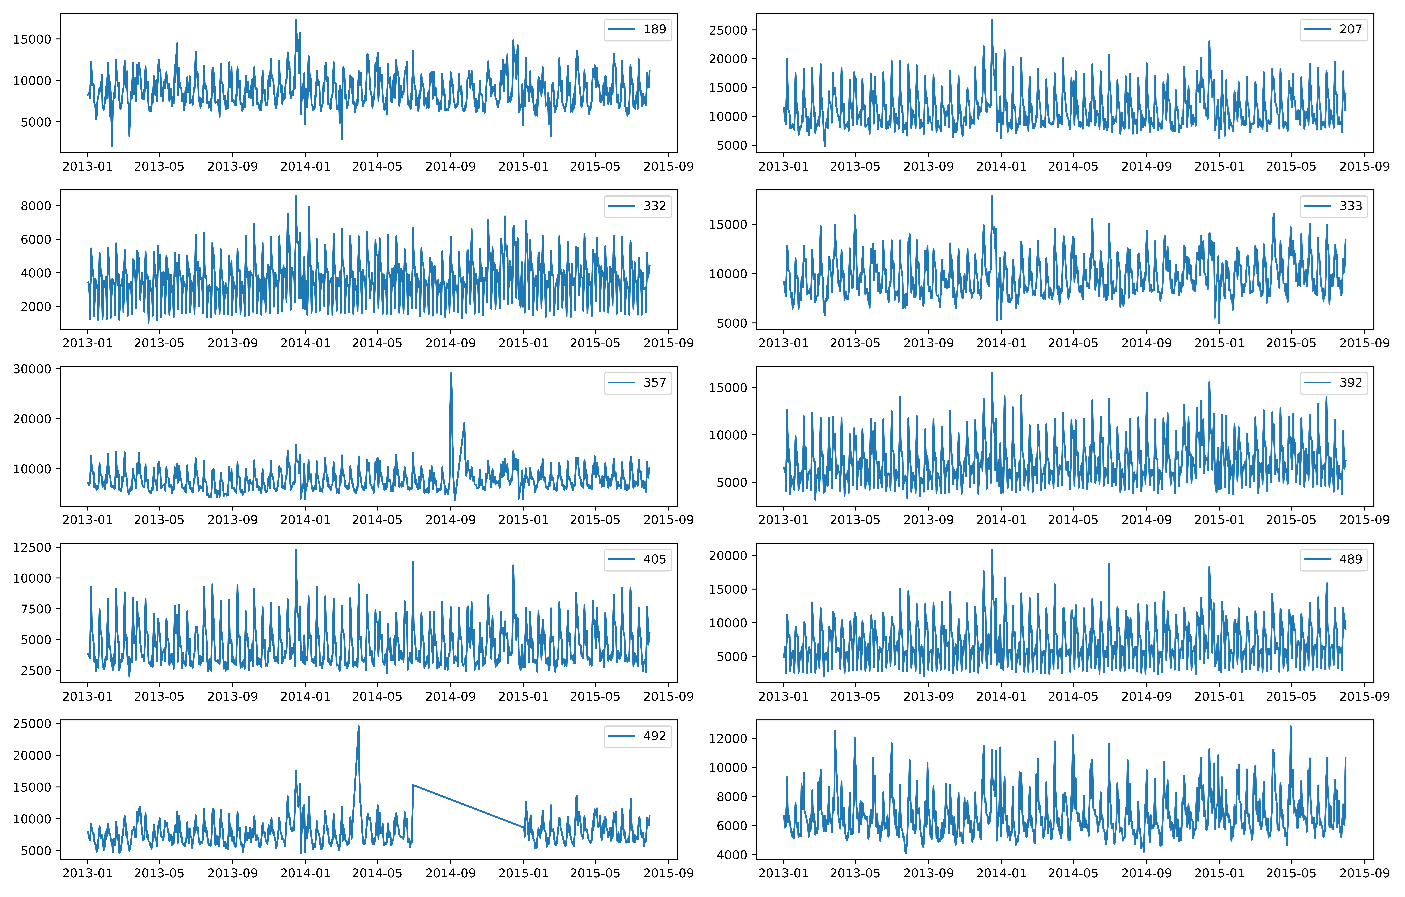
\includegraphics[scale=1.0]{Data_plot1.png}
 \label{Fig4StoreDataPlots}
 \caption{Original store data line plot}
\end{figure*}


\begin{figure*}[!h]
 \centering
 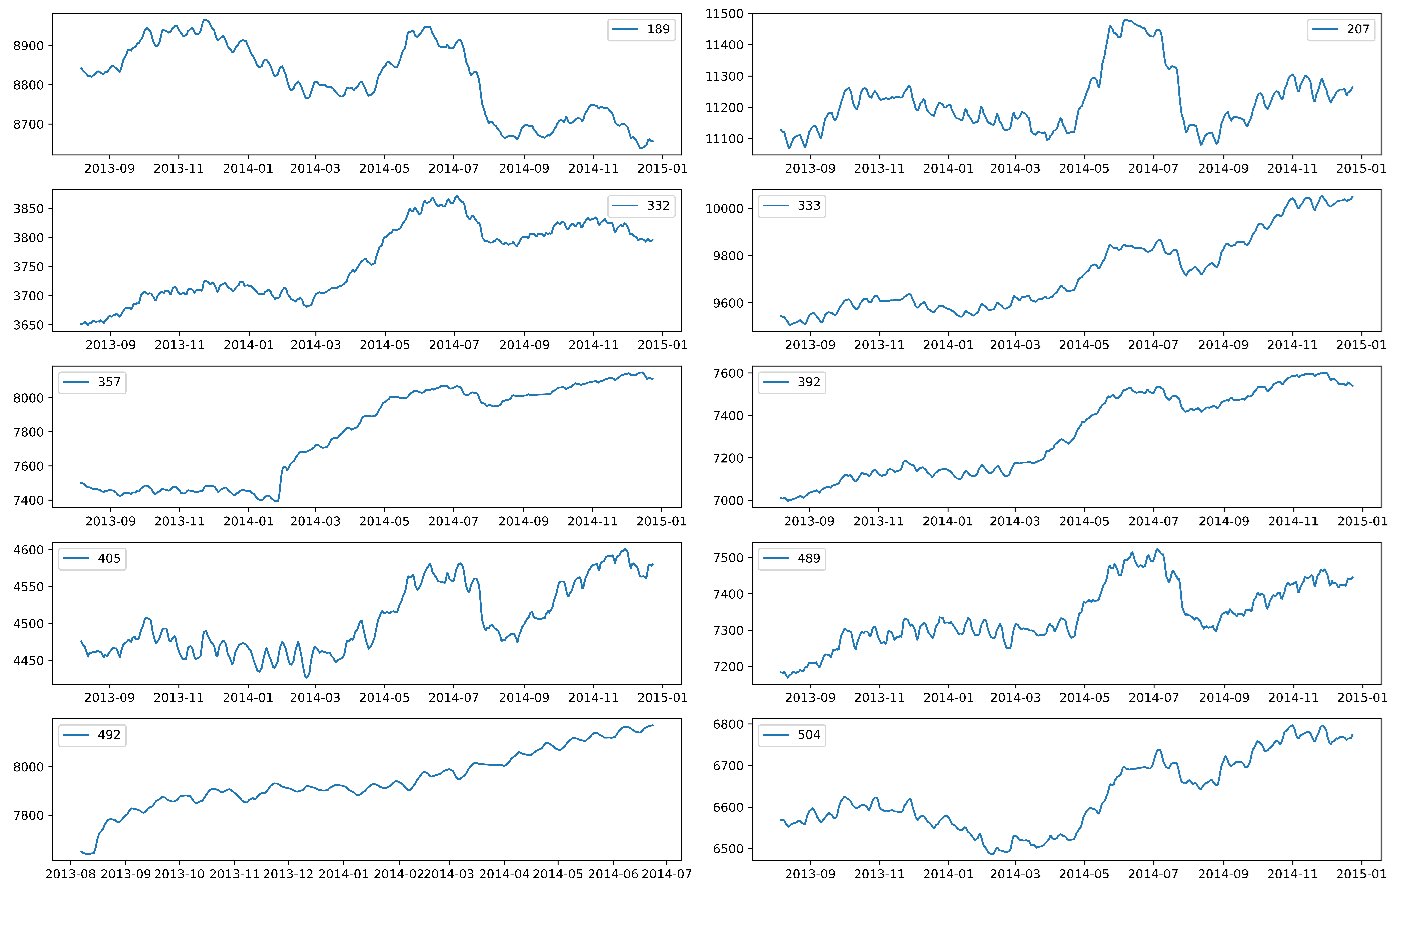
\includegraphics[scale=1.0]{data_trend1.png}
 \label{Fig5Trend}
 \caption{Trend decomposition representation of the stores data}
\end{figure*}


\begin{figure*}[!h]
 \centering
 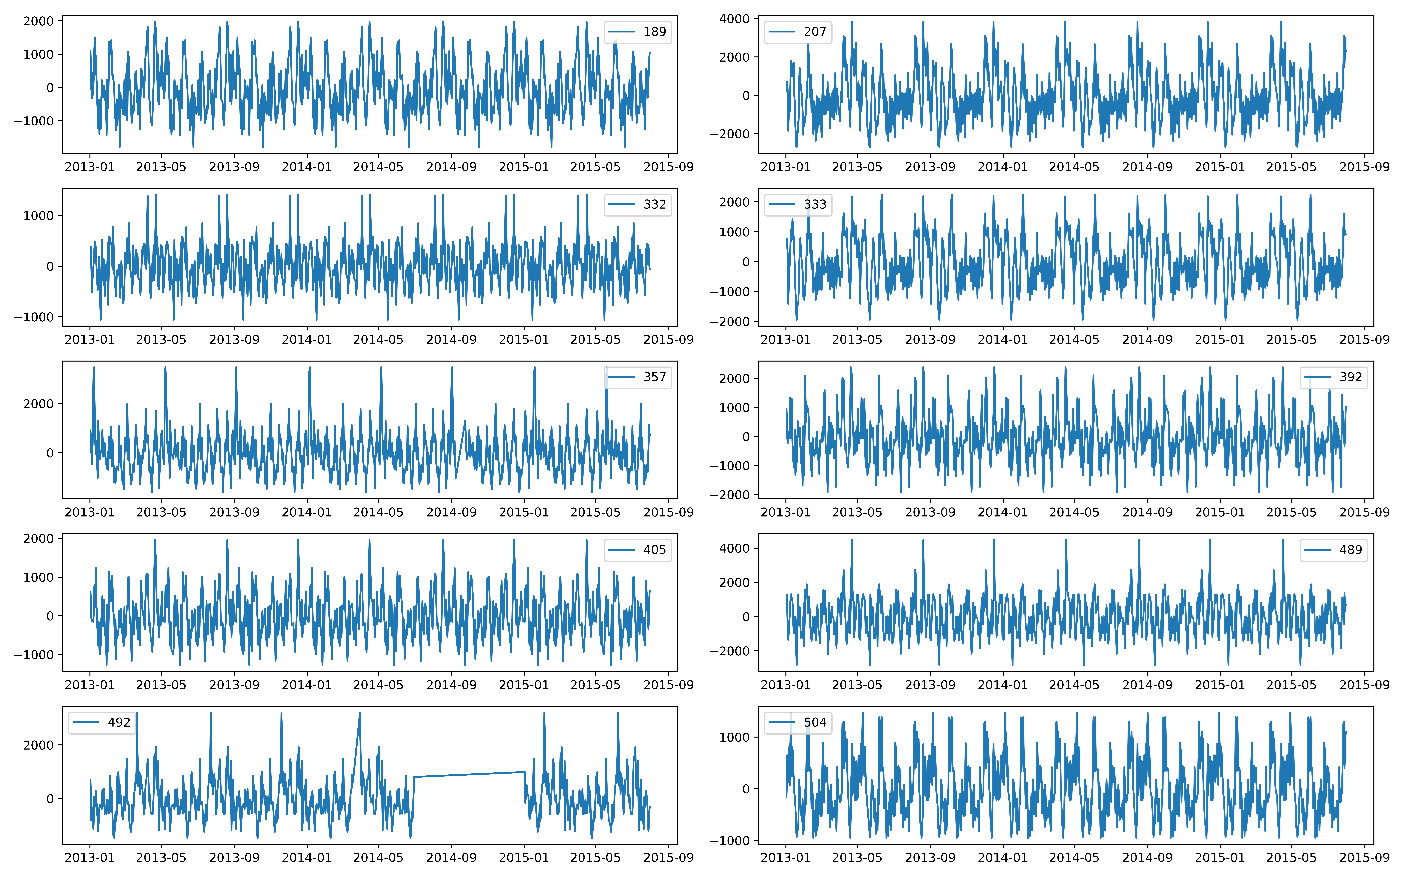
\includegraphics[scale=1.0]{data_seasonal1.png}
 \label{Fig6Seasonality}
 \caption{Seasonal decomposition representation of stores data}
\end{figure*}

%\lipsum[3-10] % Dummy text to fill space

\begin{figure*}[!h]
 \centering
 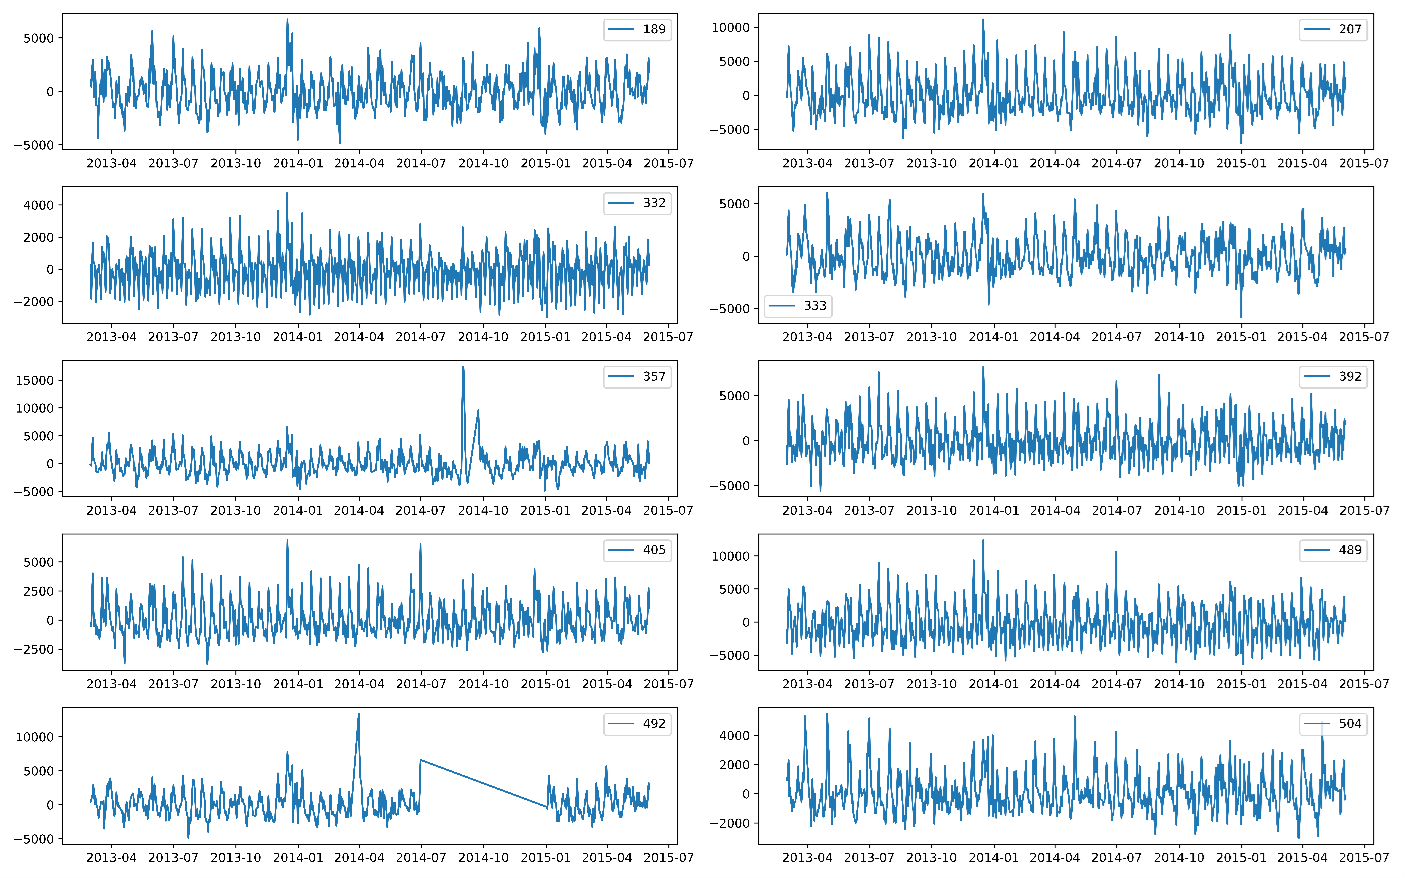
\includegraphics[scale=1.0]{data_res.png}
 \label{Fig7Residual}
 \caption{Residual decomposition representation of stores data}
\end{figure*}

